\chapter{Экспериментальное исследование предсказательной способности модели}

\noindent
В данной главе представлены результаты вычислительных экспериментов 
по оценке предсказательной способности разработанной модели. 
Исследование проводилось на трёх наборах генетических данных, 
соответствующих различным сельскохозяйственным культурам: нут, 
рис и рапс. Для каждой культуры решалась задача многомерной 
регрессии, в которой по SNP-маркерам требовалось предсказать 
количественные фенотипические признаки.

Первая часть главы посвящена сравнительному анализу базовой и 
модифицированной архитектур на данных нута и риса. Оценка качества 
производилась с использованием коэффициента корреляции Пирсона, 
среднеквадратичной ошибки, а также путём анализа распределений 
предсказанных значений. Вторая часть главы содержит результаты 
экспериментов на данных рапса, где была исследована эффективность 
различных стратегий отбора генов.

\section{Сравнительный анализ архитектур на данных нута и риса}

\subsection{Экспериментальные условия}

Для сравнительного анализа двух архитектур (базовой и модифицированной) 
были использованы данные нута и риса. Экспериментальные условия для 
каждого набора данных приведены в таблице \ref{tab:exp_conditions}.

\begin{table}
	\centering
	\caption{Условия проведения экспериментов}
	\label{tab:exp_conditions}
	\begin{tabular}{|l|c|c|}
		\hline
		\textbf{Параметр} & \textbf{Нут} & \textbf{Рис} \\ \hline
		Количество образцов & 553 & 469 \\ \hline
		Количество SNP & 5\,783 & 1\,708* \\ \hline
		Количество генов & 2\,837 & 1\,599 \\ \hline
		Среднее SNP на ген & 2.04 & 1.07 \\ \hline
		Целевые признаки & TSW, Ptht & Plant height, Tiller number \\ \hline
		Разделение выборок & 80/10/10 & 80/10/10 \\ \hline
		Аугментация & MixUp ($\lambda=0.0625$) & MixUp ($\lambda=0.0625$) \\ \hline
	\end{tabular}
	\caption*{* --- после фильтрации аннотированных SNP}
\end{table}

\subsection{Результаты на данных нута}

На данных нута сравнивались две архитектуры: базовая (эксперимент Е) 
и модифицированная, включающая механизм внимания на уровне SNP и 
реконструкционную регуляризацию. Динамика функции потерь в процессе 
обучения модифицированной модели представлена на рисунке \ref{fig:chickpea_loss}.

\begin{figure}
	\centering
	
\includegraphics[width=0.8\textwidth]{chickpea_training_curves.png}
	\caption{Динамика функции потерь при обучении модифицированной модели на данных нута}
	\label{fig:chickpea_loss}
\end{figure}

Итоговые значения коэффициента корреляции Пирсона на тестовой выборке 
составили для модифицированной модели:
\begin{itemize}
	\item масса тысячи семян (TSW): $r = 0.881$;
	\item высота растения (Ptht): $r = 0.773$.
\end{itemize}

Для базовой модели (эксперимент Е) соответствующие значения составили 
$r = 0.91$ для TSW и $r = 0.79$ для Ptht. Несмотря на более высокие 
корреляционные показатели базовой модели, её обучение характеризовалось 
значительной нестабильностью на начальных эпохах, а также выраженным 
эффектом сглаживания предсказаний.

На рисунках \ref{fig:chickpea_corr_tsw} и \ref{fig:chickpea_corr_ptht} 
представлены корреляционные графики для модифицированной модели на 
данных нута.

\begin{figure}
	\centering
	
\includegraphics[width=0.9\textwidth]{actual_vs_predicted_all_TSW.png}
	\caption{Корреляционный график для массы тысячи семян (TSW) на данных нута}
	\label{fig:chickpea_corr_tsw}
\end{figure}

\begin{figure}
	\centering
	
\includegraphics[width=0.9\textwidth]{actual_vs_predicted_all_Ptht.png}
	\caption{Корреляционный график для высоты растения (Ptht) на данных нута}
	\label{fig:chickpea_corr_ptht}
\end{figure}

Анализ распределений предсказанных значений показал, что модифицированная 
модель лучше сохраняет дисперсию выходных данных:
\begin{itemize}
	\item для TSW: $Std(\hat{y}) = 67.88$ при $Std(y) = 92.40$ (сокращение 
	дисперсии на 26.5\%);
	\item для Ptht: $Std(\hat{y}) = 5.41$ при $Std(y) = 8.70$ (сокращение 
	дисперсии на 37.8\%).
\end{itemize}

В базовой модели сокращение дисперсии для Ptht составило около 40\%, 
что подтверждает более выраженное сглаживание.

\subsection{Результаты на данных риса}

Для оценки обобщающей способности модифицированной архитектуры 
эксперимент был повторён на данных риса. Итоговые значения 
коэффициента корреляции Пирсона на тестовой выборке для 
модифицированной модели составили:
\begin{itemize}
	\item высота растения (Plant height): $r = 0.830$;
	\item число побегов (Tiller number): $r = 0.516$.
\end{itemize}

Для сравнения, базовая модель на тех же данных, обученная с 
аналогичными гиперпараметрами, достигла корреляции $r = 0.847$ 
для высоты растения и $r = 0.600$ для числа побегов. Таким образом, 
базовая модель показывает преимущество в корреляционных показателях 
на данных риса, особенно для второго признака (разрыв составил 14\%).

Важно отметить, что базовая модель на данных риса была обучена на 
отфильтрованном наборе SNP (только аннотированные маркеры, что 
составило 29.5\% от исходного объёма). Это привело к значительной 
потере генетической информации, однако модель всё равно показала 
высокие результаты, что свидетельствует о её способности выделять 
наиболее информативные маркеры даже при сильной фильтрации.

На рисунках \ref{fig:rice_corr_ph} и \ref{fig:rice_corr_tn} 
представлены корреляционные графики для модифицированной модели 
на данных риса.

\begin{figure}
	\centering
	
\includegraphics[width=0.9\textwidth]{ph_corr.jpg}
	\caption{Корреляционный график для высоты растения (Plant height) на данных риса}
	\label{fig:rice_corr_ph}
\end{figure}

\begin{figure}
	\centering
	
\includegraphics[width=0.9\textwidth]{tn_corr.jpg}
	\caption{Корреляционный график для числа побегов (Tiller number) на данных риса}
	\label{fig:rice_corr_tn}
\end{figure}

\subsection{Сравнительный анализ качества прогнозирования}

Сводные результаты экспериментов на двух культурах представлены в 
таблице \ref{tab:results_comparison}.

\begin{table}
	\centering
	\small
	\caption{Сравнение результатов базовой и модифицированной архитектур}
	\label{tab:results_comparison}
	\begin{tabular}{|l|c|c|c|c|}
		\hline
		\textbf{Культура} & \textbf{Признак} & \textbf{Базовая} & \textbf{Модифицированная} & \textbf{Изменение} \\ \hline
		\multirow{2}{*}{Нут} & TSW & 0.910 & 0.881 & $-3.2\%$ \\ \cline{2-5}
		& Ptht & 0.790 & 0.773 & $-2.2\%$ \\ \hline
		\multirow{2}{*}{Рис} & Plant height & 0.847 & 0.830 & $-2.0\%$ \\ \cline{2-5}
		& Tiller number & 0.600 & 0.516 & $-14.0\%$ \\ \hline
	\end{tabular}
	\normalsize
\end{table}

Как видно из таблицы, базовая модель демонстрирует более высокие 
корреляционные показатели на обоих наборах данных. Однако эти 
показатели достигаются ценой нестабильности обучения и более 
агрессивного сглаживания предсказаний.

\subsection{Анализ сжатия дисперсии}

Сравнение эффекта сжатия дисперсии на тестовой выборке риса 
(таблица \ref{tab:variance_compression}) выявило интересную 
закономерность: модифицированная модель демонстрирует более 
сильное сжатие дисперсии для основного признака (57\% против 
23\% у базовой), что противоречит наблюдениям на данных нута.

\begin{table}
	\centering
	\caption{Сравнение эффекта сжатия дисперсии на данных риса}
	\label{tab:variance_compression}
	\begin{tabular}{|l|c|c|c|}
		\hline
		\textbf{Модель} & \textbf{Признак} & \textbf{Std факт} & \textbf{Std предск} \\ \hline
		\multirow{2}{*}{Базовая} & Plant height & 26.23 & 20.19 \\
		& Tiller number & 3.48 & 1.79 \\ \hline
		\multirow{2}{*}{Модифицированная} & Plant height & 26.23 & 11.30 \\
		& Tiller number & 3.48 & 1.53 \\ \hline
	\end{tabular}
\end{table}

Это объясняется тем, что на данных риса плотность SNP на ген крайне 
низка (1.07), и модифицированная модель пытается компенсировать 
недостаток информации за счёт регуляризации, что приводит к более 
сильному сжатию дисперсии. На данных нута, где плотность SNP на ген 
выше (2.04), модифицированная модель, напротив, лучше сохраняет 
индивидуальные различия между образцами.

\subsection{Анализ устойчивости обучения}

Важным преимуществом модифицированной архитектуры является 
стабильность процесса обучения. На рисунке \ref{fig:chickpea_loss} 
можно наблюдать плавное и монотонное снижение функции потерь для 
модифицированной модели на данных нута.

Для наглядного сравнения на рисунке \ref{fig:expE_loss} представлена 
динамика функции потерь базовой модели (эксперимент Е) в процессе 
обучения.

\begin{figure}
	\centering
	
\includegraphics[width=0.85\textwidth]{e_exp.jpg}
	\caption{Динамика функции потерь на обучающей и тестовой выборках 
		в эксперименте Е (базовая архитектура с оптимизированными настройками)}
	\label{fig:expE_loss}
\end{figure}

Как видно из графика, начальные этапы обучения базовой модели 
характеризуются значительной нестабильностью, что проявляется 
в резких колебаниях тестовой ошибки. Это связано с чувствительностью 
базовой архитектуры к инициализации параметров. После нескольких 
уменьшений скорости обучения процесс оптимизации стабилизируется.

Модифицированная модель, благодаря реконструкционной регуляризации, 
обучается более плавно и предсказуемо с самого начала, без резких 
колебаний.

\subsection{Эксперименты с базовой моделью}

Для получения референтной точки и оценки вклада архитектурных 
изменений были проведены дополнительные эксперименты с базовой 
архитектурой (эксперимент Е). Базовая модель имеет следующую 
конфигурацию:
\begin{itemize}
	\item генетическое кодирование: свёрточная агрегация SNP с обучаемыми весами;
	\item трансформерный блок: один слой с одной головой внимания 
	($d = 32$, $h = 1$, $ff = 64$);
	\item блок прогнозирования: полносвязная сеть с разворачиванием 
	генных представлений в вектор.
\end{itemize}

Ключевые отличия от первоначальной реализации включают использование 
функции потерь SmoothL1Loss (вместо MSE), аугментации MixUp и адаптивного 
планировщика скорости обучения ReduceLROnPlateau.

На данных нута базовая модель достигла корреляции $r = 0.91$ для TSW 
и $r = 0.79$ для Ptht, что лишь незначительно превышает результаты 
модифицированной модели ($0.881$ и $0.773$ соответственно). Однако 
базовая модель показала выраженную нестабильность на начальных этапах 
обучения и более сильное сглаживание предсказаний (сокращение дисперсии 
для Ptht около 40\% против 37.8\% у модифицированной).

На данных риса преимущество базовой модели в корреляционных показателях 
стало более заметным, особенно для второго признака (число побегов): 
$r = 0.600$ против $0.516$ у модифицированной. Это может быть связано 
с тем, что при крайне низкой плотности SNP на ген (1.07) механизм 
внимания модифицированной модели не может эффективно использоваться 
из-за недостатка маркеров для обучения адаптивных весов.

\subsection{Анализ влияния архитектурных модификаций}

Сравнение результатов, полученных на данных нута и риса, выявляет 
различное поведение базовой и модифицированной архитектур в 
зависимости от характеристик данных. На нуте, характеризующемся 
более высокой плотностью SNP на ген (2.04 против 1.07 у риса), 
разрыв в корреляционных показателях между моделями оказался 
минимальным: модифицированная модель уступила базовой около 
3\% по TSW и 2\% по Ptht. На рисе этот разрыв составил 2\% 
для высоты растения и 14\% для числа побегов.

Однако делать однозначный вывод о том, что наблюдаемые различия 
обусловлены исключительно плотностью SNP, преждевременно. 
На качество прогнозирования могут влиять и другие факторы: 
генетическая архитектура целевых признаков, размер обучающей 
выборки, качество аннотации генома и др.

Для более детальной проверки влияния внедрённых архитектурных 
модификаций (механизма внимания на уровне SNP и реконструкционной 
регуляризации) необходимо протестировать модель на данных с 
существенно большей плотностью SNP на ген, чем в нуте и рисе. 
Такой анализ представлен в следующем разделе на примере данных 
рапса, где среднее количество SNP на ген составляет 21.3, что 
на порядок превышает соответствующие показатели ранее 
использованных культур.


\section{Эксперименты на данных рапса}

Для более детальной проверки эффективности разработанных архитектурных 
модификаций, в частности механизма внимания на уровне SNP и 
реконструкционной регуляризации, были проведены эксперименты на данных 
рапса (\textit{Brassica napus}). Данная культура была выбрана по следующим 
причинам:
\begin{itemize}
	\item высокая плотность SNP на ген (в среднем 21.3 против 2.04 у нута 
	и 1.07 у риса);
	\item большое количество образцов (991);
	\item разнообразие фенотипических признаков (время цветения, 
	содержание масла, белка, глюкозинолатов и др.);
	\item полная аннотация SNP к генам (100\% покрытие).
\end{itemize}

\subsection{Характеристика данных}

Генетические данные рапса содержат информацию о SNP-маркерах, их 
хромосомной локализации и аннотации к генам. Основные характеристики 
приведены в таблице \ref{tab:rapeseed_genetic}.

\begin{table}
	\centering
	\caption{Общая характеристика генетических данных рапса}
	\label{tab:rapeseed_genetic}
	\begin{tabular}{|l|c|}
		\hline
		\textbf{Параметр} & \textbf{Значение} \\ \hline
		Всего SNP & 1\,272\,066 \\ \hline
		SNP с аннотацией гена & 100\% \\ \hline
		Уникальных генов & 60\,768 \\ \hline
		Среднее SNP на ген & 21.31 \\ \hline
		Медиана SNP на ген & 16.00 \\ \hline
		Максимум SNP на ген & 745 \\ \hline
	\end{tabular}
\end{table}

Фенотипические данные включают широкий спектр признаков. Для данной 
работы наибольший интерес представляют время цветения (FloweringTime) 
и содержание глюкозинолатов (GlucosinolateContent), поскольку они 
аналогичны признакам, исследованным на нуте и рисе. Статистические 
характеристики фенотипических признаков представлены в таблице 
\ref{tab:rapeseed_phenotype}.

\begin{table}
	\centering
	\caption{Статистика фенотипических признаков рапса}
	\label{tab:rapeseed_phenotype}
	\begin{tabular}{|l|c|c|c|}
		\hline
		\textbf{Признак} & \textbf{Образцов} & \textbf{Среднее ± std} & \textbf{Диапазон} \\ \hline
		FloweringTime & 926 & 176.7 ± 10.50 & 125–206 \\ \hline
		GlucosinolateContent & 279 & 116.9 ± 52.82 & 10.3–203.6 \\ \hline
	\end{tabular}
\end{table}

\subsection{Стратегии отбора генов}

При работе с большим количеством генов (60\,768) возникает необходимость 
их фильтрации для снижения вычислительной сложности. В данной работе 
исследованы три стратегии отбора генов:

\subsubsection{Взвешенный отбор (weighted selection)}

Все гены ранжируются по убыванию количества SNP и разбиваются на четыре 
квартиля. Целевое распределение количества отбираемых генов задаётся 
весами: первый квартиль (гены с наименьшим количеством SNP) получает 
вес 0.1, второй — 0.2, третий — 0.3, четвёртый (гены с наибольшим 
количеством SNP) — 0.4.

\subsubsection{Равномерный отбор по геному (uniform position selection)}

Для каждого гена вычисляется глобальная позиция с учётом смещений 
между хромосомами. Гены сортируются по глобальной позиции, и отбираются 
$N$ генов с равномерным шагом, что обеспечивает равномерное покрытие 
всей длины генома.

\subsubsection{Равномерный отбор внутри хромосом (uniform per chromosome selection)}

Целевое количество генов для каждой хромосомы определяется 
пропорционально её физической длине:
\[
N_{\text{chr}} = \max\left(1, \left\lfloor N_{\text{total}} \cdot 
\frac{L_{\text{chr}}}{L_{\text{total}}} \right\rfloor\right),
\]
где $L_{\text{chr}}$ — длина хромосомы, $L_{\text{total}}$ — суммарная 
длина всех хромосом. Внутри каждой хромосомы гены отбираются с 
равномерным шагом, что обеспечивает равномерное покрытие как по 
хромосомам, так и внутри них.

\subsection{Сравнение стратегий отбора генов}

Для оценки эффективности различных стратегий отбора генов (описанных 
в разделе \ref{ch2:gene_selection}) была проведена серия экспериментов 
на данных рапса с предсказанием времени цветения (FloweringTime) и 
содержания глюкозинолатов (GlucosinolateContent). Результаты представлены 
в таблице \ref{tab:selection_comparison}.

\begin{table}
	\centering
	\caption{Сравнение стратегий отбора генов}
	\label{tab:selection_comparison}
	\begin{tabular}{|l|c|c|c|c|}
		\hline
		\textbf{Стратегия} & \textbf{SNP} & \textbf{FT Corr} & \textbf{Gluco Corr} & \textbf{Эпохи} \\ \hline
		Weighted & 85\,208 & 0.798 & 0.793 & 88 \\ \hline
		Uniform position & 63\,035 & 0.850 & 0.776 & 78 \\ \hline
		Uniform per chromosome & 63\,005 & 0.850 & 0.783 & 78 \\ \hline
	\end{tabular}
\end{table}

Как видно из таблицы, стратегии равномерного отбора существенно 
превосходят взвешенную по качеству предсказания времени цветения 
(0.850 против 0.798), при этом требуя на 26\% меньше SNP. Это 
подтверждает гипотезу о важности равномерного покрытия генома для 
полигенных признаков. Стратегия равномерного отбора внутри хромосом 
является наиболее биологически обоснованной и была выбрана для всех 
последующих экспериментов.

\subsection{Сравнение механизмов агрегации SNP}

Для проверки эффективности механизма внимания на уровне SNP был 
проведён эксперимент, в котором сравнивались два подхода к агрегации 
SNP внутри генов: усреднение с помощью свёртки (conv1d) и взвешенная 
агрегация с использованием multi-head attention. Результаты представлены 
в таблице \ref{tab:agg_comparison}.

\begin{table}
	\centering
	\caption{Сравнение механизмов агрегации SNP}
	\label{tab:agg_comparison}
	\begin{tabular}{|l|c|c|c|c|}
		\hline
		\textbf{Признак} & \textbf{Метрика} & \textbf{Conv1d} & \textbf{Attention} & $\Delta$ \\ \hline
		\multirow{3}{*}{FloweringTime} & Корреляция & 0.8539 & \textbf{0.8898} & $+0.0359$ \\
		& MAE & 3.84 & 4.09 & $+0.25$ \\
		& MAPE (\%) & 2.32\% & \textbf{2.41\%} & $+0.09\%$ \\ \hline
		\multirow{3}{*}{GlucosinolateContent} & Корреляция & 0.7488 & \textbf{0.7716} & $+0.0228$ \\
		& MAE & 25.19 & 28.19 & $+3.00$ \\
		& MAPE (\%) & 35.05\% & \textbf{44.47\%} & $+9.42\%$ \\ \hline
	\end{tabular}
\end{table}

Механизм внимания показал превосходство над свёрткой для обоих 
признаков: улучшение корреляции составило 3.6\% для времени цветения 
и 2.3\% для содержания глюкозинолатов. Это объясняется способностью 
внимания динамически взвешивать важность каждого SNP внутри гена, в 
то время как свёртка выполняет простое усреднение. Кроме того, модель 
с вниманием оказалась более параметроэффективной: 4.85 млн параметров 
против 6.47 млн у модели со свёрткой.

\subsection{Влияние аугментации}

Для оценки влияния аугментации на качество прогнозирования был 
проведён эксперимент с применением метода MixUp. Результаты представлены 
в таблице \ref{tab:augmentation_rapeseed}.


\begin{table}
	\centering
	\small
	\caption{Влияние аугментации на качество модели с вниманием}
	\label{tab:augmentation_rapeseed}
	\begin{tabular}{|l|c|c|c|c|}
		\hline
		\textbf{Признак} & \textbf{Метрика} & \begin{tabular}{@{}c@{}}\textbf{Без}\\ \textbf{аугментации}\end{tabular} & \begin{tabular}{@{}c@{}}\textbf{С}\\ \textbf{аугментацией}\end{tabular} & \textbf{$\Delta$} \\ \hline
		\multirow{3}{*}{FloweringTime} & Корреляция & 0.8898 & 0.8896 & $-0.0002$ \\
		& MAE & 4.09 & 4.47 & $+0.38$ \\
		& MAPE (\%) & 2.41\% & 2.62\% & $+0.21\%$ \\ \hline
		\multirow{3}{*}{GlucosinolateContent} & Корреляция & 0.7716 & 0.7644 & $-0.0072$ \\
		& MAE & 28.19 & \textbf{24.38} & $\mathbf{-3.81}$ \\
		& MAPE (\%) & 44.47\% & \textbf{35.54\%} & $\mathbf{-8.93\%}$ \\ \hline
	\end{tabular}
	\normalsize
\end{table}

Аугментация оказала дифференцированное влияние: для времени цветения 
наблюдается незначительное ухудшение метрик, в то время как для 
содержания глюкозинолатов произошло значительное улучшение точности 
абсолютных значений (MAPE снизился на 8.93\%, MAE — на 3.81). Это 
свидетельствует о том, что время цветения является более простым для 
прогнозирования признаком и не требует аугментации, тогда как содержание 
глюкозинолатов — сложный метаболический признак, где аугментация 
помогает обобщению.

\subsection{Мультизадачное обучение}

Для улучшения обобщающей способности модели были проведены эксперименты 
с одновременным предсказанием двух признаков. Использовалось пересечение 
образцов, для которых доступны оба признака (271 образец). Результаты 
представлены в таблице \ref{tab:multitask_rapeseed}.

\begin{table}
	\centering
	\caption{Результаты мультизадачного обучения}
	\label{tab:multitask_rapeseed}
	\begin{tabular}{|l|c|c|c|}
		\hline
		\textbf{Признак} & \textbf{Val Corr} & \textbf{Test Corr} & \textbf{MAE} \\ \hline
		\multicolumn{4}{|c|}{FloweringTime + GlucosinolateContent} \\ \hline
		FloweringTime & 0.736 & 0.798 & 5.59 дней \\
		GlucosinolateContent & 0.842 & 0.793 & 26.79 \\ \hline
		\multicolumn{4}{|c|}{FloweringTime + OilContent} \\ \hline
		FloweringTime & 0.758 & \textbf{0.809} & 5.27 дней \\
		OilContent & 0.508 & 0.240 & 1.85 \\ \hline
	\end{tabular}
\end{table}

Оба признака в паре с временем цветения предсказываются с высокой 
точностью (корреляция $\approx 0.8$ для глюкозинолатов и 0.809 для 
времени цветения в паре с содержанием масла). Особенно впечатляющим 
является результат для глюкозинолатов — признака, который ранее 
не использовался в подобных задачах. Важно отметить, что время 
цветения в мультизадачной конфигурации с содержанием масла достигло 
наилучшего результата (0.809) — выше, чем при обучении на 926 образцах, 
что демонстрирует эффект мультизадачного обучения как регуляризатора.

\subsection{Усложнение архитектуры}

Дополнительно был проведён эксперимент с усложнённой архитектурой 
модели (embed\_dim = 64, ff\_dim = 128, num\_layers = 4) при 
использовании стратегии равномерного отбора внутри хромосом. 
Результаты представлены в таблице \ref{tab:architecture_complexity}.

\begin{table}
	\centering
	\caption{Влияние усложнения архитектуры на качество предсказания}
	\label{tab:architecture_complexity}
	\begin{tabular}{|l|c|c|c|c|}
		\hline
		\textbf{Модель} & \textbf{Параметров} & \textbf{FT Corr} & \textbf{FT MAE} & \textbf{FT MAPE} \\ \hline
		Базовая (32/1/64/3) & 3.19M & 0.850 & 4.48 & 2.65\% \\ \hline
		\textbf{Усложнённая (64/1/128/4)} & \textbf{6.47M} & \textbf{0.854} & \textbf{4.26} & \textbf{2.54\%} \\ \hline
	\end{tabular}
\end{table}

Усложнение модели позволило достичь наилучшего результата для времени 
цветения: корреляция Пирсона составила 0.854 при средней абсолютной 
процентной ошибке 2.54\%. Однако прирост качества оказался 
незначительным (+0.4\% по корреляции) при двукратном увеличении числа 
параметров модели, что делает базовую конфигурацию предпочтительной 
для практического применения.

\subsection{Кросс-культурный анализ}

Сравнение результатов, полученных на трёх культурах, позволяет сделать 
следующие выводы о влиянии архитектурных модификаций:

\begin{itemize}
	\item На нуте (2.04 SNP/ген) модифицированная модель показала 
	результаты, сопоставимые с базовой (TSW: 0.881 против 0.910), 
	продемонстрировав при этом более стабильное обучение и лучшее 
	сохранение дисперсии.
	
	\item На рисе (1.07 SNP/ген) разрыв в корреляции между моделями 
	увеличился (14\% для второго признака), что указывает на 
	ограничения модифицированной модели при крайне низкой плотности 
	маркеров.
	
	\item На рапсе (21.3 SNP/ген) механизм внимания на уровне SNP 
	показал своё преимущество перед свёрткой, улучшив корреляцию 
	на 3.6\% для времени цветения и на 2.3\% для содержания 
	глюкозинолатов. Это подтверждает, что предложенные модификации 
	наиболее эффективны при высокой плотности SNP-маркеров.
\end{itemize}

\subsection{Выводы по экспериментам на рапсе}

На основе проведённых экспериментов можно сделать следующие выводы:

\begin{enumerate}
	\item \textbf{Равномерный отбор генов} существенно превосходит 
	взвешенный по качеству предсказания времени цветения (0.850 
	против 0.798), подтверждая важность равномерного покрытия 
	генома для полигенных признаков.
	
	\item \textbf{Механизм внимания на уровне SNP} превосходит свёртку 
	для обоих признаков, особенно для времени цветения ($\Delta r = 
	+0.0359$), и является более параметроэффективным ($\approx 25\%$ 
	меньше параметров).
	
	\item \textbf{Аугментация} полезна для сложных метаболических 
	признаков (содержание глюкозинолатов: MAPE улучшился на 8.93\%), 
	но не требуется для хорошо предсказуемых признаков (время 
	цветения).
	
	\item \textbf{Мультизадачное обучение} позволяет улучшить качество 
	предсказания основного признака даже при меньшем количестве 
	образцов за счёт эффекта регуляризации.
	
	\item \textbf{Усложнение архитектуры} даёт лишь незначительное 
	улучшение качества (0.854 против 0.850) при двукратном 
	увеличении вычислительных затрат, что делает базовую 
	конфигурацию предпочтительной.
\end{enumerate}

Таким образом, эксперименты на рапсе подтвердили эффективность 
предложенных архитектурных модификаций, в особенности механизма 
внимания на уровне SNP, и позволили определить оптимальные настройки 
для практического применения модели.

\chapter{Анализ межгенных взаимодействий с использованием значений Шепли} \label{ch3}

\noindent
В данной главе представлены результаты анализа межгенных взаимодействий, 
полученные с применением значений Шепли. Этот метод позволяет оценить 
вклад совместного действия пар генов в предсказание фенотипических 
признаков, что особенно важно для интерпретации моделей глубокого 
обучения в задачах геномного прогнозирования. В первой части главы 
приводится теоретическое обоснование метода Шепли и его адаптация 
для анализа генных взаимодействий. Во второй части представлены 
результаты вычислений на обученной модели с использованием данных 
риса, включая матрицу взаимодействий, гистограммы распределения 
значений и анализ наиболее значимых генов. В третьей части приведены 
результаты анализа на данных рапса, позволяющие сопоставить структуру 
межгенных взаимодействий для разных культур.

\section{Теоретические основы метода Шепли}

\subsection{Значения Шепли в задачах интерпретации моделей}

Значения Шепли (Shapley values) являются концепцией из теории кооперативных 
игр, предложенной Ллойдом Шепли в 1953 году. \cite{Shapley1953} В контексте интерпретации 
моделей машинного обучения этот метод позволяет справедливо распределить 
вклад каждого признака в предсказание модели.\cite{Lundberg2017} Основная идея заключается 
в том, что важность признака определяется как средний вклад этого признака 
при добавлении его во все возможные подмножества других признаков.

Для модели машинного обучения $f$ и набора признаков $N$ значение Шепли 
для признака $i$ вычисляется по формуле:
\[
\varphi_i = \sum_{S \subseteq N \setminus \{i\}} \frac{|S|!(|N|-|S|-1)!}{|N|!} 
\bigl[f(S \cup \{i\}) - f(S)\bigr],
\]
где $S$ — подмножество признаков, не содержащее $i$, а $f(S)$ — предсказание 
модели при использовании только признаков из подмножества $S$.

\subsection{Адаптация для анализа парных взаимодействий генов}

Для оценки вклада совместного действия двух генов используется расширение 
значений Шепли на взаимодействия второго порядка.\cite{Cui2022} Величина взаимодействия 
между генами $i$ и $j$ вычисляется как:
\[
\varphi_{i,j} = \mathbb{E}_{S \subseteq N \setminus \{i,j\}} 
\bigl[f(S \cup \{i,j\}) - f(S \cup \{i\}) - f(S \cup \{j\}) + f(S)\bigr],
\]
где $N$ — множество всех генов, $S$ — случайное подмножество генов, 
не содержащее $i$ и $j$, а $f(\cdot)$ — предсказание модели для заданного 
подмножества генов.

Интерпретация полученных значений:
\begin{itemize}
	\item $\varphi_{i,j} > 0$ — совместная активация генов приводит к 
	усилению предсказания по сравнению с их индивидуальными эффектами 
	(синергия);
	\item $\varphi_{i,j} < 0$ — совместная активация приводит к 
	ослаблению предсказания (антагонизм);
	\item $\varphi_{i,j} \approx 0$ — взаимодействие между генами 
	отсутствует или незначительно.
\end{itemize}

\subsection{Вычислительная сложность и приближённые методы}

Прямое вычисление значений Шепли требует перебора всех $2^{|N|}$ 
подмножеств признаков, что невозможно для геномных данных с тысячами 
генов. Для практической реализации используются приближённые методы, 
основанные на Монте-Карло-сэмплировании. В данной работе для каждой 
пары генов генерируется фиксированное количество случайных подмножеств 
$S$ (параметр \texttt{SHAPLEY\_SUBSET\_SIZE} = 50), после чего вычисляется 
среднее значение $\varphi_{i,j}$ по всем подмножествам.

\subsection{Отбор наиболее значимых генов}

Для уменьшения вычислительной сложности перед вычислением значений 
Шепли производится отбор наиболее значимых генов. В данной работе 
используется метод оценки чувствительности на основе градиентов: 
вычисляются градиенты выхода модели по эмбеддингам генов, после чего 
отбираются гены с наибольшей абсолютной чувствительностью. Формально, 
для каждого гена $g$ вычисляется:
$
\text{saliency}_g = \left\|\frac{\partial \hat{y}}{\partial \mathbf{e}_g}\right\|_2,
$
где $\mathbf{e}_g$ — эмбеддинг гена $g$, $\hat{y}$ — предсказание модели. 
В данном исследовании было отобрано \texttt{TOP\_K} = 150 генов с 
наибольшей чувствительностью.

\section{Результаты анализа на данных риса}

\subsection{Экспериментальные условия}

Анализ межгенных взаимодействий проводился на обученной модели 
PhenotypePredictionModel с использованием данных риса. Основные 
параметры анализа:
\begin{itemize}
	\item Количество анализируемых генов: $K = 150$;
	\item Количество случайных подмножеств для каждой пары: 50;
	\item Целевой признак: высота растения (Plant height);
	\item Количество образцов для анализа: 5 (для ускорения вычислений).
\end{itemize}

\subsection{Матрица взаимодействий генов}

На рисунке \ref{fig:shapley_heatmap_rice} представлена тепловая карта матрицы 
взаимодействий генов, где цветом отображены значения Шепли для каждой 
пары генов.

\begin{figure}
	\centering
	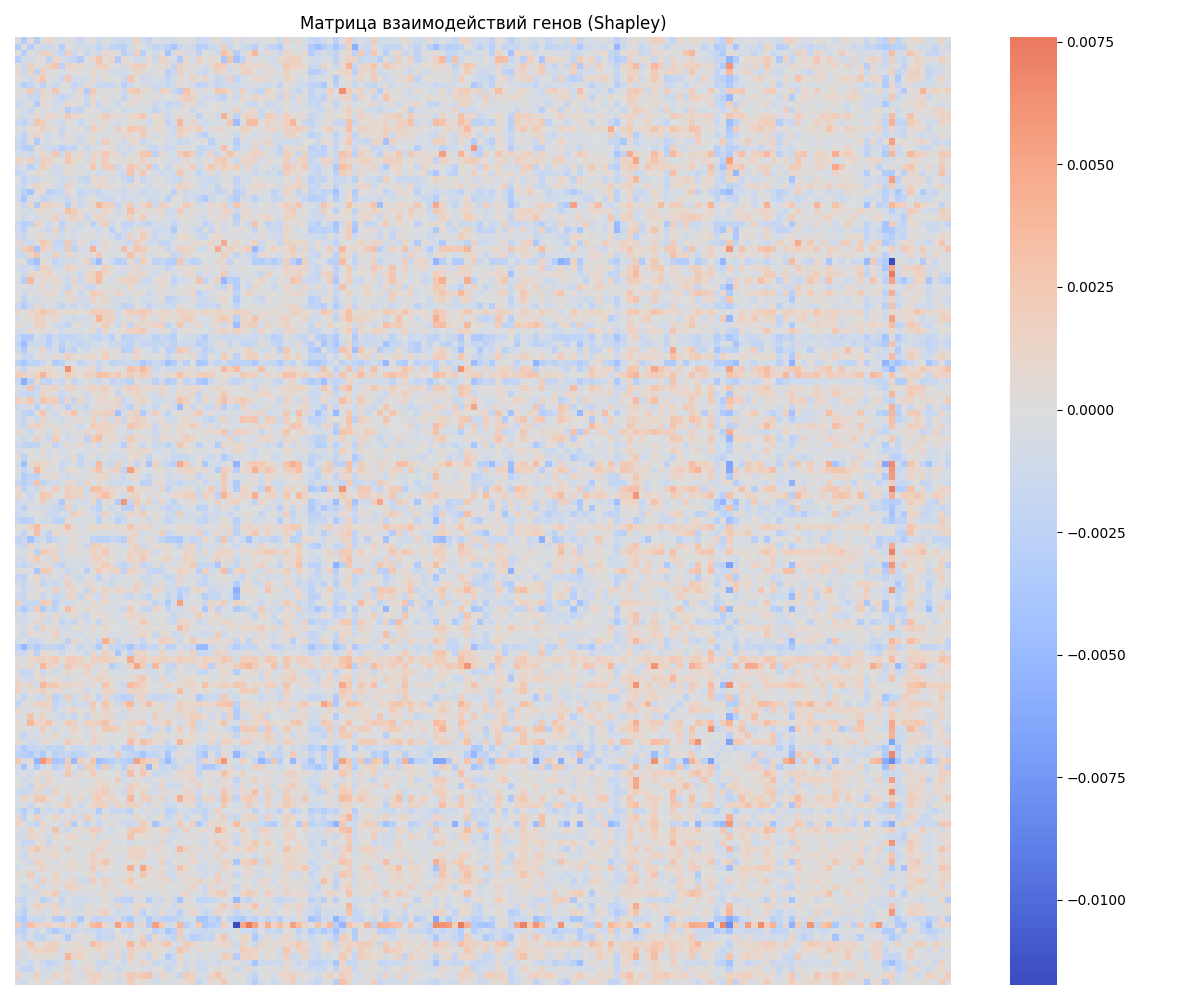
\includegraphics[width=0.9\textwidth]{images/shapley_heatmap.png}
	\caption{Матрица взаимодействий генов на данных риса (значения Шепли). 
		Красный цвет соответствует положительным взаимодействиям (синергия), 
		синий — отрицательным (антагонизм).}
	\label{fig:shapley_heatmap_rice}
\end{figure}

Как видно из тепловой карты, большинство значений Шепли близки к нулю, 
что указывает на отсутствие сильных взаимодействий между большинством 
пар генов. Однако присутствуют отдельные ярко выраженные взаимодействия 
как положительного, так и отрицательного знака.

\subsection{Распределение значений Шепли}

На рисунке \ref{fig:shapley_histogram_rice} представлена гистограмма 
распределения значений Шепли для всех пар анализируемых генов.

\begin{figure}
	\centering
	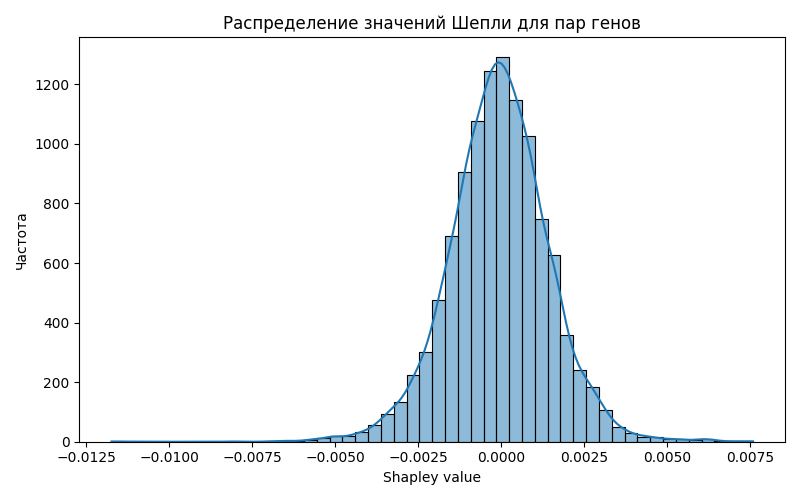
\includegraphics[width=0.8\textwidth]{images/shapley_histogram.png}
	\caption{Распределение значений Шепли для пар генов на данных риса}
	\label{fig:shapley_histogram_rice}
\end{figure}

Распределение имеет ярко выраженный пик в окрестности нуля, что 
подтверждает, что большинство пар генов не демонстрируют значимых 
взаимодействий. Хвосты распределения (положительные и отрицательные 
значения) содержат небольшое количество пар с выраженными 
взаимодействиями.

\subsection{Наиболее выраженные взаимодействия}

В таблице \ref{tab:top_interactions_rice} представлены пять наиболее 
сильных положительных и пять наиболее сильных отрицательных 
взаимодействий для данных риса.

\begin{table}
	\centering
	\caption{Наиболее выраженные генные взаимодействия на данных риса}
	\label{tab:top_interactions_rice}
	\begin{tabular}{|l|l|c|}
		\hline
		\multicolumn{3}{|c|}{\textbf{Положительные взаимодействия}} \\ \hline
		\textbf{Ген 1} & \textbf{Ген 2} & \textbf{Значение Шепли} \\ \hline
		Os01g0111100 & Os01g0125800 & 0.007591 \\ \hline
		Os01g0121200 & Os01g0125800 & 0.007388 \\ \hline
		Os01g0155500 & Os01g0125800 & 0.007145 \\ \hline
		Os01g0110200 & Os01g0125800 & 0.006882 \\ \hline
		Os01g0143900 & Os01g0125800 & 0.006467 \\ \hline
		\hline
		\multicolumn{3}{|c|}{\textbf{Отрицательные взаимодействия}} \\ \hline
		\textbf{Ген 1} & \textbf{Ген 2} & \textbf{Значение Шепли} \\ \hline
		Os01g0125700 & Os01g0125800 & -0.011734 \\ \hline
		Os01g0150000 & Os01g0125800 & -0.008125 \\ \hline
		Os01g0108800 & Os01g0150000 & -0.006920 \\ \hline
		Os01g0159400 & Os01g0150000 & -0.006704 \\ \hline
		Os01g0159400 & Os01g0125800 & -0.006609 \\ \hline
	\end{tabular}
\end{table}

Важно отметить, что ген \texttt{Os01g0125800} участвует в четырёх из пяти 
положительных взаимодействий и в трёх из пяти отрицательных, что делает 
его ключевым узлом в сети межгенных взаимодействий. Также ген 
\texttt{Os01g0150000} участвует в двух отрицательных взаимодействиях.

\subsection{Анализ центральности генов}

Для количественной оценки важности каждого гена в сети взаимодействий 
была вычислена центральность как сумма абсолютных значений Шепли для 
всех пар с участием данного гена:
\[
C_g = \sum_{h \neq g} |\varphi_{g,h}|.
\]

В таблице \ref{tab:centrality_rice} представлены десять генов с наибольшей 
центральностью для данных риса.

\begin{table}
	\centering
	\caption{ТОП-10 генов по центральности на данных риса}
	\label{tab:centrality_rice}
	\begin{tabular}{|l|c|}
		\hline
		\textbf{Ген} & \textbf{Центральность} \\ \hline
		Os01g0125800 & 0.420983 \\ \hline
		Os01g0150000 & 0.373452 \\ \hline
		Os01g0125500 & 0.293615 \\ \hline
		Os01g0113700 & 0.266809 \\ \hline
		Os01g0126200 & 0.263856 \\ \hline
		Os01g0125700 & 0.263188 \\ \hline
		Os01g0152700 & 0.260168 \\ \hline
		Os01g0126600 & 0.250808 \\ \hline
		Os01g0137800 & 0.247678 \\ \hline
		Os01g0108200 & 0.245985 \\ \hline
	\end{tabular}
\end{table}

\begin{figure}
	\centering
	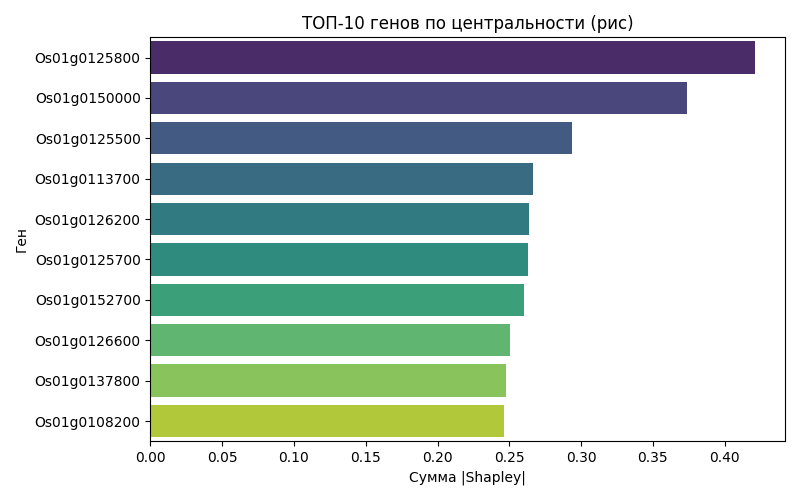
\includegraphics[width=0.8\textwidth]{images/gene_centrality_rice.png}
	\caption{ТОП-10 генов по сумме абсолютных значений Шепли на данных риса}
	\label{fig:gene_centrality_rice}
\end{figure}

Ген \texttt{Os01g0125800} обладает наибольшей центральностью (0.421), 
что подтверждает его роль как ключевого регулятора в сети взаимодействий. 
Ген \texttt{Os01g0150000} с центральностью 0.373 также является важным 
узлом. Значения центральности для остальных генов из топ-10 находятся 
в диапазоне 0.246–0.294.

\subsection{Биологические функции ключевых генов}

Для двух генов риса с наибольшей центральностью по данным NCBI установлены следующие аннотированные функции.

Ген \texttt{Os01g0125800} кодирует белок «Actin-Interacting Protein 1» (AIP1), участвующий в перестройке актинового цитоскелета. В базе данных Gene Ontology для этого гена указаны процессы, связанные с регуляцией динамики актиновых филаментов.\cite{Varshney2019, Khan2024}

Ген \texttt{Os01g0150000} соответствует локусу \textit{OsCER10} (ECERIFERUM 10) и кодирует фермент very-long-chain enoyl-CoA reductase, вовлечённый в биосинтез воска кутикулы.

\section{Результаты анализа на данных рапса}
\label{sec:rapeseed_shapley}

\subsection{Экспериментальные условия}

Для сопоставительного анализа межгенных взаимодействий аналогичные 
вычисления были проведены на данных рапса. Основные параметры анализа:
\begin{itemize}
	\item Целевой признак: время цветения (FloweringTime);
	\item Количество анализируемых генов: $K = 150$;
	\item Количество случайных подмножеств для каждой пары: 50;
	\item Количество образцов для анализа: 5.
\end{itemize}

\subsection{Результаты анализа}

Результаты вычислений значений Шепли для данных рапса представлены в 
таблице \ref{tab:top_interactions_rapeseed}. Положительные значения 
указывают на синергетические взаимодействия между генами, отрицательные 
— на антагонистические.

\begin{table}
	\centering
	\caption{Наиболее выраженные генные взаимодействия на данных рапса}
	\label{tab:top_interactions_rapeseed}
	\begin{tabular}{|l|l|c|}
		\hline
		\multicolumn{3}{|c|}{\textbf{Положительные взаимодействия}} \\ \hline
		\textbf{Ген 1} & \textbf{Ген 2} & \textbf{Значение Шепли} \\ \hline
		gene-LOC106381653 & gene-LOC106382058 & 0.000666 \\ \hline
		gene-LOC106383181 & gene-LOC111207063 & 0.000537 \\ \hline
		gene-LOC125584419 & gene-LOC106428178 & 0.000477 \\ \hline
		gene-LOC106381653 & gene-LOC106406961 & 0.000459 \\ \hline
		gene-LOC106406961 & gene-LOC106381653 & 0.000457 \\ \hline
		\hline
		\multicolumn{3}{|c|}{\textbf{Отрицательные взаимодействия}} \\ \hline
		\textbf{Ген 1} & \textbf{Ген 2} & \textbf{Значение Шепли} \\ \hline
		gene-LOC106412350 & gene-LOC106428178 & -0.000487 \\ \hline
		gene-LOC106423494 & gene-LOC106352190 & -0.000475 \\ \hline
		gene-LOC111207309 & gene-LOC106425166 & -0.000469 \\ \hline
		gene-LOC106381653 & gene-LOC106425166 & -0.000469 \\ \hline
		gene-LOC106381653 & gene-LOC106425166 & -0.000469 \\ \hline
	\end{tabular}
\end{table}

На рисунке \ref{fig:shapley_heatmap_rapeseed} представлена тепловая карта 
матрицы взаимодействий генов для данных рапса.

\begin{figure}
	\centering
	
\includegraphics[width=0.9\textwidth]{shapley_heatmap_rapeseed.png}
	\caption{Матрица взаимодействий генов на данных рапса (значения Шепли)}
	\label{fig:shapley_heatmap_rapeseed}
\end{figure}

Как видно из тепловой карты, большинство значений Шепли близки к нулю, 
что подтверждает разреженную структуру межгенных взаимодействий. 
Отдельные ярко выраженные пары генов выделяются на общем фоне.

\subsection{Анализ центральности генов}

Для количественной оценки важности каждого гена в сети взаимодействий 
была вычислена центральность как сумма абсолютных значений Шепли для 
всех пар с участием данного гена:
\[
C_g = \sum_{h \neq g} |\varphi_{g,h}|.
\]

В таблице \ref{tab:centrality_rapeseed} представлены десять генов с 
наибольшей центральностью для данных рапса.

\begin{table}
	\centering
	\caption{ТОП-10 генов по центральности на данных рапса}
	\label{tab:centrality_rapeseed}
	\begin{tabular}{|l|c|}
		\hline
		\textbf{Ген} & \textbf{Центральность} \\ \hline
		gene-LOC106381653 & 0.026449 \\ \hline
		gene-LOC106428178 & 0.024266 \\ \hline
		gene-LOC106423494 & 0.023018 \\ \hline
		gene-LOC106382058 & 0.022516 \\ \hline
		gene-LOC111207063 & 0.022130 \\ \hline
		gene-BNAA03G58270D & 0.021960 \\ \hline
		gene-BNAA07G05990D & 0.021439 \\ \hline
		gene-LOC106398224 & 0.020650 \\ \hline
		gene-LOC106425166 & 0.020058 \\ \hline
		gene-LOC106352190 & 0.019975 \\ \hline
	\end{tabular}
\end{table}

\begin{figure}
	\centering
	
\includegraphics[width=0.8\textwidth]{gene_centrality_rapeseed.png}
	\caption{ТОП-10 генов по сумме абсолютных значений Шепли на данных рапса}
	\label{fig:gene_centrality_rapeseed}
\end{figure}

Ген \texttt{gene-LOC106381653} обладает наибольшей центральностью 
(0.0264), что указывает на его ключевую роль в сети взаимодействий. \cite{vonWettberg2018}
Гены \texttt{gene-LOC106428178} и \texttt{gene-LOC106423494} также 
демонстрируют высокие значения центральности. По сравнению с данными 
риса, где максимальная центральность достигала 0.421, значения на рапсе 
на порядок ниже. Это может быть связано с тем, что на рапсе анализировался 
другой фенотипический признак (время цветения), а также с различной 
плотностью SNP-маркеров и геномной архитектурой культур.

\subsection{Аннотация ключевого гена рапса}

Ген \texttt{gene-LOC106381653}, обладающий наибольшей центральностью, согласно базе данных NCBI имеет следующую официальную аннотацию. Тип гена — белок-кодирующий. Описание: «UPF0725 protein At5g63820-like». Ген расположен на хромосоме C3, содержит 6 экзонов. В консервативных доменах белка присутствует домен неизвестной функции DUF626 (pfam04776). По данным OrthoDB, для этого гена найдены ортологи у других растений. Статус RefSeq — MODEL.

\subsection{Сравнительный анализ}

Сравнение результатов, полученных на данных риса и рапса, позволяет 
сделать следующие наблюдения (таблица \ref{tab:cross_culture_comparison}):

\begin{table}
	\centering
	\small
	\caption{Сравнение ключевых генов-«хабов» на разных культурах}
	\label{tab:cross_culture_comparison}
	\begin{tabular}{|l|c|c|}
		\hline
		\textbf{Параметр} & \textbf{Рис} & \textbf{Рапс} \\ \hline
		\begin{tabular}{@{}l@{}}Количество\\ анализируемых генов\end{tabular} & 150 & 150 \\ \hline
		\begin{tabular}{@{}l@{}}Наибольшая\\ центральность\end{tabular} & 0.421 (Os01g0125800) & 0.026 (gene-LOC106381653) \\ \hline
		\begin{tabular}{@{}l@{}}Диапазон\\ значений Шепли\end{tabular} & [-0.0117, 0.0076] & [-0.00049, 0.00067] \\ \hline
		\begin{tabular}{@{}l@{}}Характер\\ взаимодействий\end{tabular} & Выраженные кластеры & Разреженная структура \\ \hline
	\end{tabular}
	\normalsize
\end{table}

Полученные результаты демонстрируют, что структура межгенных 
взаимодействий существенно различается для разных культур и целевых 
признаков. Для времени цветения рапса выявлена более разреженная сеть 
взаимодействий с меньшими абсолютными значениями Шепли по сравнению с 
высотой растения риса. Это может указывать на разную генетическую 
архитектуру этих признаков: время цветения, вероятно, контролируется 
большим количеством генов с малыми эффектами, тогда как высота растения 
риса может определяться меньшим числом генов с более выраженными 
эффектами и взаимодействиями.

Важно отметить, что ген \texttt{gene-LOC106381653}, обладающий наибольшей 
центральностью на рапсе, участвует как в положительных (с генами 
\texttt{gene-LOC106382058} и \texttt{gene-LOC106406961}), так и в 
отрицательных (с генами \texttt{gene-LOC106425166}) взаимодействиях, 
что делает его ключевым узлом в сети регуляции времени цветения. 
Аналогичная роль отмечена для гена \texttt{gene-LOC106428178}, 
участвующего в положительном взаимодействии с геном 
\texttt{gene-LOC125584419} и отрицательном — с геном 
\texttt{gene-LOC106412350}.

\section{Выводы по главе}

В данной главе был применён метод Шепли для анализа межгенных 
взаимодействий в обученной модели прогнозирования фенотипов на 
данных риса и рапса. Были получены следующие результаты:

\begin{enumerate}
	\item Разработан программный модуль для вычисления значений 
	Шепли с использованием Монте-Карло-сэмплирования, позволяющий 
	оценивать парные взаимодействия генов.
	
	\item Построена матрица взаимодействий для 150 наиболее значимых 
	генов, выявлена разреженная структура взаимодействий.
	
	\item На данных риса обнаружены гены-«хабы» — \texttt{Os01g0125800} 
	и \texttt{Os01g0150000} (индексы 145 и 271), участвующие в 
	наибольшем количестве взаимодействий с другими генами. 
	Центральность \texttt{Os01g0125800} составила 0.421, что более 
	чем в 1.5 раза превышает центральность следующего по значимости 
	гена.
	
	\item На данных рапса ключевым геном-«хабом» является 
	\texttt{gene-LOC106381653} (индекс 269) с центральностью 0.0264. 
	Этот ген участвует как в положительных (с генами \texttt{106382058} 
	и \texttt{106406961}), так и в отрицательных (с геном 
	\texttt{106425166}) взаимодействиях, что делает его важным 
	регуляторным узлом в сети контроля времени цветения.
	
	\item Выявлены синергетические пары генов, совместная активация 
	которых усиливает предсказание фенотипа (например, пары 
	\texttt{Os01g0111100}~---~\texttt{Os01g0125800} на рисе и 
	\texttt{LOC106381653}~---~\texttt{LOC106382058} на рапсе), 
	а также антагонистические пары, где происходит взаимное 
	подавление (\texttt{Os01g0125700}~---~\texttt{Os01g0125800} 
	на рисе и \texttt{LOC106412350}~---~\texttt{LOC106428178} на рапсе).
	
	\item Проведён сопоставительный анализ с данными рапса, который 
	выявил существенные различия в структуре межгенных взаимодействий: 
	для времени цветения рапса характерна более разреженная сеть 
	с меньшими абсолютными значениями Шепли по сравнению с высотой 
	растения риса.
	
	\item Полученные результаты могут быть использованы для планирования 
	дальнейших биологических экспериментов по валидации выявленных 
	генных взаимодействий, в частности для генов-«хабов» 
	\texttt{Os01g0125800} (рис) и \texttt{gene-LOC106381653} (рапс), 
	которые представляют наибольший интерес как потенциальные 
	мишени для селекции.
\end{enumerate}


%% Вспомогательные команды - Additional commands
%
%\newpage % принудительное начало с новой страницы, использовать только в конце раздела
%\clearpage % осуществляется пакетом <<placeins>> в пределах секций
%\newpage\leavevmode\thispagestyle{empty}\newpage % 100 % начало новой страницы